\documentclass[aspectratio=169,10pt]{beamer}
\usepackage{amsmath,amssymb,booktabs,graphicx}
\usepackage[T1]{fontenc}
\usepackage{lmodern}

\definecolor{navy}{HTML}{132A46}
\definecolor{blue}{HTML}{2374AB}
\definecolor{teal}{HTML}{2A9D8F}
\definecolor{gold}{HTML}{E9A23B}
\definecolor{soft}{HTML}{F3F6F8}
\definecolor{ink}{HTML}{263238}
\setbeamercolor{normal text}{fg=ink,bg=white}
\setbeamercolor{structure}{fg=blue}
\setbeamercolor{frametitle}{fg=white,bg=navy}
\setbeamercolor{title}{fg=white}
\setbeamercolor{subtitle}{fg=white!82}
\setbeamercolor{block title}{fg=white,bg=blue}
\setbeamercolor{block body}{fg=ink,bg=soft}
\setbeamercolor{alerted text}{fg=gold!80!black}
\setbeamertemplate{navigation symbols}{}
\setbeamertemplate{itemize item}{\color{teal}$\blacktriangleright$}
\setbeamertemplate{itemize subitem}{\color{blue}$\bullet$}
\setbeamertemplate{footline}{%
  \leavevmode\hbox{%
  \begin{beamercolorbox}[wd=.86\paperwidth,ht=2.7ex,dp=1.2ex,leftskip=1em]{author in head/foot}%
    \color{navy}\scriptsize MTH 9871 \;|\; Arbitrage-Free Implied Volatility
  \end{beamercolorbox}%
  \begin{beamercolorbox}[wd=.14\paperwidth,ht=2.7ex,dp=1.2ex,center]{date in head/foot}%
    \color{navy}\scriptsize \insertframenumber/\inserttotalframenumber
  \end{beamercolorbox}}}
\setbeamertemplate{frametitle}{\vspace{0.25em}\hspace{0.35em}\insertframetitle\vspace{0.25em}}
\setbeamersize{text margin left=0.65cm,text margin right=0.65cm}

\newcommand{\metric}[2]{%
  \begin{beamercolorbox}[rounded=true,sep=.55em,center,wd=\linewidth]{block body}
    {\color{navy}\Large\bfseries #1}\\[-0.1em]
    {\scriptsize #2}
  \end{beamercolorbox}}

\title{Arbitrage-Free Implied Volatility\\and Temporal Filtering}
\subtitle{Full-Day NVDA OPRA-Style Analysis}
\author{Chaithanya Pakala}
\institute{MTH 9871 \;\textbullet\; Instructor: Beat Ammon}
\date{Lecture 3 Assignment}

\begin{document}

\begin{frame}[plain]
  \begin{beamercolorbox}[wd=\paperwidth,ht=\paperheight,dp=0ex]{frametitle}
    \vspace{1.15cm}\hspace{1.05cm}
    \begin{minipage}{0.82\paperwidth}
      {\color{teal}\rule{2.0cm}{2.5pt}}\\[0.65cm]
      {\color{white}\fontsize{25}{29}\selectfont\bfseries\inserttitle\par}
      \vspace{0.4cm}
      {\color{white!82}\large\insertsubtitle\par}
      \vfill
      {\color{white}\normalsize\insertauthor\par}
      {\color{white!72}\small\insertinstitute\par}
      \vspace{1.0cm}
    \end{minipage}
  \end{beamercolorbox}
\end{frame}

\begin{frame}{Problem, Data, and Scope}
\begin{columns}[T,onlytextwidth]
\column{0.57\textwidth}
\textbf{Assignment goals}
\begin{itemize}
  \item Fit a short-dated smile to a \alert{full day of real quotes}.
  \item Enforce call monotonicity, convexity, and the endogenous Roger Lee bound during optimization.
  \item Test the fit one minute ahead; report spread misses, MSE, bias, and ATM ACF.
  \item Extend the fit with constrained Kalman temporal smoothing.
\end{itemize}
\column{0.40\textwidth}
\begin{block}{Selected market slice}
\begin{tabular}{@{}ll@{}}
Underlying & NVDA\\
Trade date & 2024-10-14\\
Expiry & 2024-11-15\\
Snapshots & 390 (09:31--16:00)\\
Raw rows & 176,280\\
Fit quotes & 52,205\\
Maturity & 0.088411 years
\end{tabular}
\end{block}
\vspace{0.25em}
\small Forward inferred each minute from robust call--put parity; OTM puts are converted to call-equivalent prices below the forward.
\end{columns}
\end{frame}

\begin{frame}{Pricing and Implied-Volatility Inversion}
\begin{columns}[T,onlytextwidth]
\column{0.51\textwidth}
\begin{block}{Forward Black--Scholes call}
\begin{align*}
C(K)&=D\!F\,[F\Phi(d_1)-K\Phi(d_2)],\\
d_{1,2}&=\frac{\log(F/K)\pm\tfrac12\sigma^2\tau}{\sigma\sqrt{\tau}}.
\end{align*}
\end{block}
\begin{itemize}
  \item Brent root search on $\sigma\in[10^{-5},5]$.
  \item Reject prices outside intrinsic and upper bounds.
  \item Short-dated continuously compounded rate proxy: $r=4.8\%$.
\end{itemize}
\column{0.46\textwidth}
\vspace{0.2cm}
\metric{PASS}{price $\rightarrow$ IV $\rightarrow$ price recovery}
\vspace{0.5cm}
\begin{block}{Market-data safeguards}
\small Uncrossed, finite quotes only; at least eight usable strikes per minute. Actual run: 133--134 strikes per snapshot. OTM selection mitigates deep-ITM staleness and American early-exercise effects.
\end{block}
\end{columns}
\end{frame}

\begin{frame}{Endogenous Roger Lee Bound in SNS Space}
Let $k=\log(K/F)$, total variance $\omega=\tau v$, ATM volatility $a=\sqrt{v(0)}$, and
\[s=\frac{k}{a\sqrt{\tau}}.\]
Then the chain rule gives
\[
\frac{\partial\omega}{\partial k}
=\tau\frac{\partial v}{\partial s}\frac{\partial s}{\partial k}
=\frac{\sqrt{\tau}}{a}v'(s).
\]
Therefore $|\partial_k\omega|\le 2$ becomes
\[
\boxed{|v'(s)|\le \frac{2\sqrt{v(0)}}{\sqrt{\tau}}}
\quad\Longleftrightarrow\quad
[v'(s)]^2\le\frac{4}{\tau}v(0).
\]
\begin{block}{Why no outer bootstrap is needed}
The ATM level remains a function of the fitted coefficients. Squaring produces a rotated second-order-cone form, enforced jointly with $v(s)>0$ rather than plugging in a fixed ATM estimate.
\end{block}
\end{frame}

\begin{frame}{Constrained Curve Fit}
\begin{columns}[T,onlytextwidth]
\column{0.47\textwidth}
Fit annualized variance on $s\in[-3.5,3.5]$:
\[v(s)=\beta_0+\beta_1s+\beta_2s^2+\beta_3s^3+\beta_4s^4.\]
\textbf{Constraints inside every SLSQP fit}
\begin{itemize}
  \item $v(s)\ge 0.0004$ on the fit grid;
  \item endogenous Lee slope inequality;
  \item call slopes in $[-1,0]$;
  \item nondecreasing call slopes (convexity).
\end{itemize}
Warm starts use the prior minute, but infeasible optimizer output is never accepted.
\column{0.50\textwidth}
\metric{390 / 390}{optimizer solutions accepted}
\vspace{0.35cm}
\metric{$4.168\times10^{-5}$}{minimum dense-grid constraint margin}
\vspace{0.35cm}
\metric{PASS}{monotonicity, convexity, Lee, and finite-difference checks}
\end{columns}
\end{frame}

\begin{frame}{Representative Real-Market Smile}
\begin{columns}[T,onlytextwidth]
\column{0.72\textwidth}
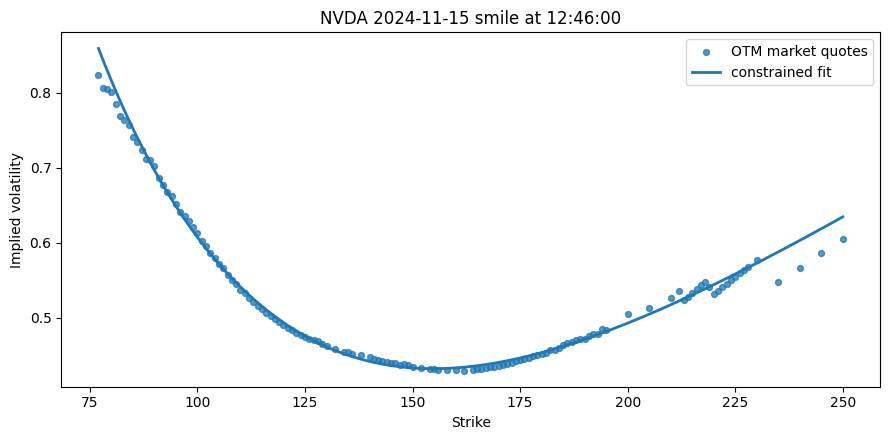
\includegraphics[width=\linewidth]{presentation_assets/nvda_smile.png}
\column{0.25\textwidth}
\small
\textbf{12:46 snapshot}
\begin{itemize}
  \item Strong left skew and curved wings are visible.
  \item The fit tracks the liquid center closely.
  \item Constraints apply only over the local SNS domain.
\end{itemize}
\begin{block}{Dense-grid result}
Call slope range:\\
$[-0.993639,-0.000726]$\\[0.2em]
Minimum convexity increment:\\
$1.980\times10^{-5}$
\end{block}
\end{columns}
\end{frame}

\begin{frame}{One-Minute-Ahead Out-of-Sample Test}
At minute $t+1$, revalue its strikes and parity-implied forward using coefficients fitted only at minute $t$.
\vspace{0.35cm}
\begin{columns}[T,onlytextwidth]
\column{0.23\textwidth}\metric{52,072}{held-out quote comparisons}
\column{0.23\textwidth}\metric{55.32\%}{predictions outside bid/offer}
\column{0.23\textwidth}\metric{0.02342}{price RMSE}
\column{0.23\textwidth}\metric{$-0.00033$}{signed price bias}
\end{columns}
\vspace{0.55cm}
\begin{block}{Interpretation}
The error is effectively unbiased and small in dollar-price units, but narrow one-minute spreads make the outside-spread test demanding. The statistic measures executable quote agreement, not only in-sample variance loss. Price MSE is $5.48\times10^{-4}$.
\end{block}
\end{frame}

\begin{frame}{Extension A: Constrained Kalman Smoothing}
\begin{columns}[T,onlytextwidth]
\column{0.34\textwidth}
\small
State and observation equations:
\[
\beta_t=\beta_{t-1}+\epsilon_t,
\qquad y_t=B(s_t)\beta_t+\eta_t.
\]
The textbook posterior is projected in its precision metric onto the same no-arbitrage feasible set.
\begin{itemize}
  \item Identity transition; state = five coefficients.
  \item SNS locations frozen at predicted ATM.
  \item \alert{389/389} constrained projections succeeded.
  \item Slack constraints reproduce the textbook posterior exactly: max error $0.0$.
\end{itemize}
\column{0.63\textwidth}
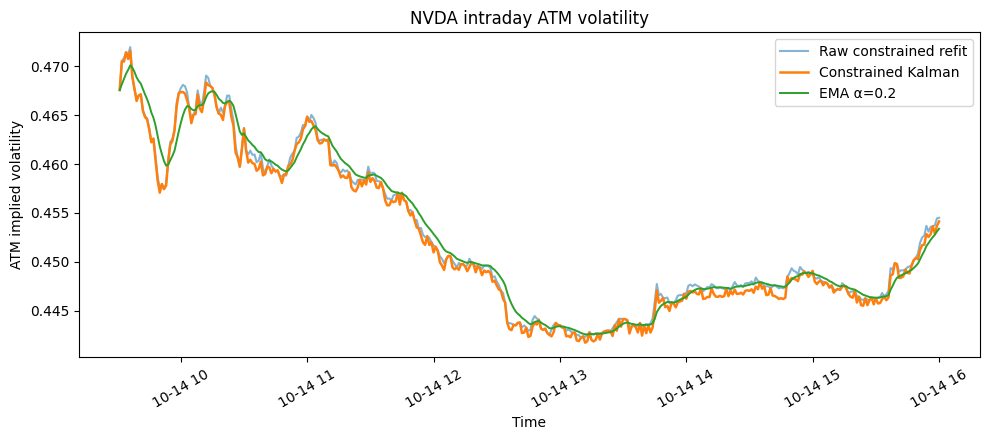
\includegraphics[width=\linewidth]{presentation_assets/nvda_atm_timeseries.png}
\end{columns}
\end{frame}

\begin{frame}{Persistence, Practical Value, and Limits}
\begin{columns}[T,onlytextwidth]
\column{0.57\textwidth}
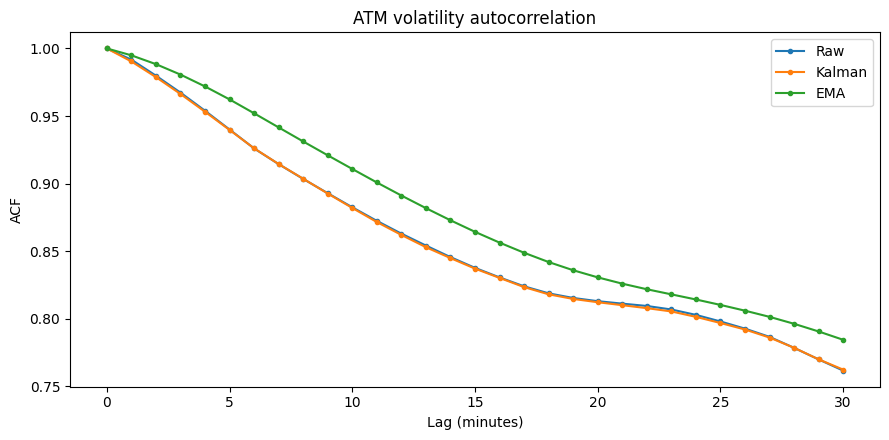
\includegraphics[width=\linewidth]{presentation_assets/nvda_atm_acf.png}
\column{0.40\textwidth}
\small
\textbf{Selected ATM ACF}
\begin{center}
\begin{tabular}{@{}rrrr@{}}
\toprule
Lag & Raw & Kalman & EMA\\
\midrule
1  & .9917 & .9904 & .9949\\
5  & .9400 & .9397 & .9623\\
15 & .8377 & .8371 & .8643\\
30 & .7617 & .7624 & .7845\\
\bottomrule
\end{tabular}
\end{center}
\textbf{Market-making value:} steadier quotes, Greeks, hedges, and inventory marks using the whole smile.

\textbf{Costs/limits:} covariance calibration, projection cost, lag at jumps, local SNS linearization, European approximation for American NVDA options, and finite-grid rather than global guarantees.
\end{columns}
\end{frame}

\end{document}
